% -------------------------------------------------------------------------------- %

\begin{exercise}[Exercise 8.1]

The nonplanning method looks particularly poor in Figure \ref{fig:8.3} because it is a one-step method;
a method using multi-step bootstrapping would do better.
Do you think one of the multi-step bootstrapping methods from Chapter 7 could do as well as the Dyna method?
Explain why or why not.

\setcounter{section}{8}
\setcounter{figure}{2}

\begin{figure}[H]
    \centering
    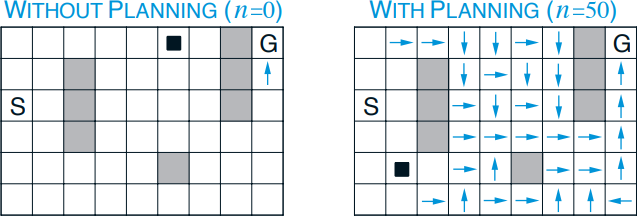
\includegraphics[width = 0.5 \textwidth]{4.45.png}
    \caption
    {
        Policies found by planning and nonplanning Dyna-Q agents halfway through the second episode.
        The arrows indicate the greedy action in each state;
        if no arrow is shown for a state, then all of its action values were equal.
        The black square indicates the location of the agent.
    }
    \label{fig:8.3}
\end{figure}

\end{exercise}

% -------------------------------------------------------------------------------- %

\begin{solution}

\phantom{}

\end{solution}

% -------------------------------------------------------------------------------- %
